Das Ziel des Abschnitts «Methoden und Materialien» ist es, dem Leser die Gelegenheit zu bieten, alle Phasen des Versuchs reproduzieren zu können.

\begin{itemize}
    \item[-] Beschreiben Sie Ihre Herangehensweise inklusive Arbeitsaufteilung und den Ablauf des Versuchs. Zitieren Sie dabei jeweils zusätzlich verwendete Ressourcen [8] und referenzieren Sie diese im Literaturverzeichnis.
    \item[-] Listen Sie alle genutzten Geräte [9] und Software [2] und referenzieren Sie jeweils deren Dokumentation im Literaturverzeichnis.
\end{itemize}

\gls{latex} wird oft für wissenschaftliche Arbeiten genutzt. \gls{ai} ist ein Teilbereich von \gls{ml}. Zweite Verwendung von \gls{ai} und \gls{ml}. Test \gls{bfh}.


Hier wird ein Werk zitiert.\cite{EinsteinCoefficientsSpringerLink}

Hie rwird ein weiteres Werk zitiert.\cite{5GrundlagenFur2025}

% ----------------- Bilder -----------------
\begin{figure}[H]
    \centering
    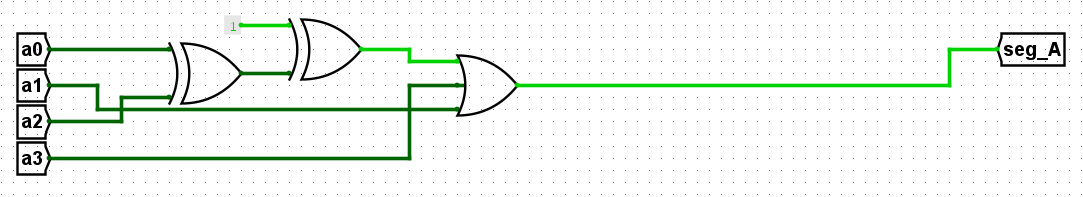
\includegraphics[width=1\textwidth]{segment_A.png}
    \caption{Logikschaltung Segment A}
    \label{fig:segment_A}
\end{figure}

Die Logikschaltung zum Segment A wurde wie in Abbildung~\ref{fig:segment_A} gezeigt aufgebaut.

\begin{figure}[H]
    \centering
    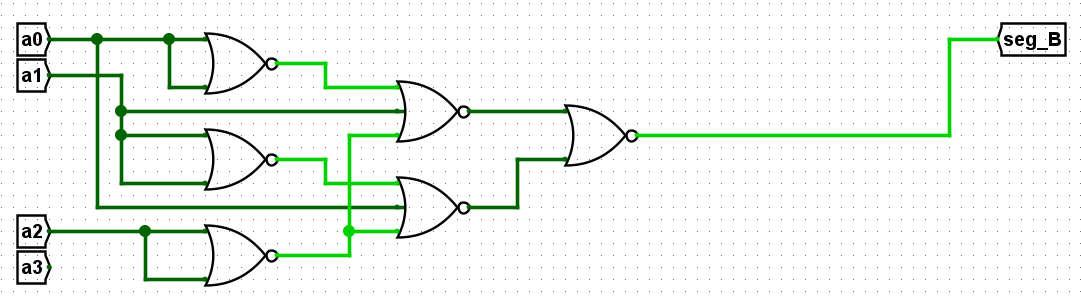
\includegraphics[width=1\textwidth]{segment_B.png}
    \caption{Logikschaltung Segment B}
    \label{fig:segment_B}
\end{figure}

Die Logikschaltung zum Segment B wurde wie in Abbildung~\ref{fig:segment_B} gezeigt aufgebaut.

\begin{figure}[H]
    \centering
    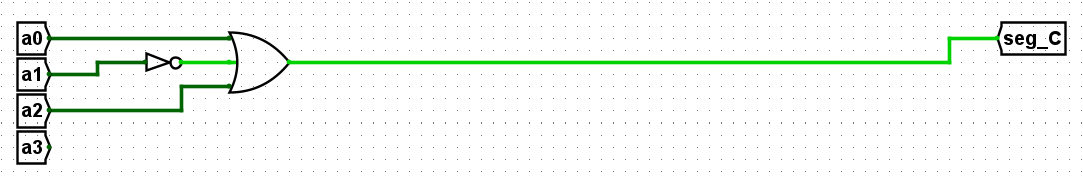
\includegraphics[width=1\textwidth]{segment_C.png}
    \caption{Logikschaltung Segment C}
    \label{fig:segment_C}
\end{figure}

Die Logikschaltung zum Segment C wurde wie in Abbildung~\ref{fig:segment_C} gezeigt aufgebaut.

% ----------------- Tabelle -----------------
\vspace{1em} % Abstand
Nachfolgend die Wahrheitstabelle der Segmente:
\begin{table}[ht]
\centering
\colorlet{BFH-table}{BFH-MediumBlue!10}
\colorlet{BFH-tablehead}{BFH-MediumBlue!50}
\setupBfhTabular
\begin{bfhTabular}{llllllllllll}
Input & a3 & a2 & a1 & a0 & seg\_A & seg\_B & seg\_C & seg\_D & seg\_E & seg\_F & seg\_G \\\hline
\num{0} & \num{0} & \num{0} & \num{0} & \num{0} & \num{1} & \num{1} & \num{1} & \num{1} & \num{1} & \num{1} & \num{0} \\\hline
\num{1} & \num{0} & \num{0} & \num{0} & \num{1} & \num{0} & \num{1} & \num{1} & \num{0} & \num{0} & \num{0} & \num{0} \\\hline
\end{bfhTabular}
\caption{Wahrheitstabelle Siebensegmentanzeige}
\label{tab:truthtable_bcd_to_7segment}
\end{table}